\section{Framework and API}
\ewu{I feel like we should use "\sys model " more consistently}
This section describes how we model machine learning prediction and the \sys problem.
Let the training dataset $D$ contain tuples of features $x_i$ and labels $y_i$ that are categorical or real-valued.
\texttt{train(D)} is a training algorithm that returns a model \texttt{model($\cdot$)} that takes as input a test point $x_{new}$ and predicts a label $\hat{y}_{new}$:
\[
\hat{y}_{new} = \textsf{model}(x_{new})
\]

\vspace{0.5em}\noindent \textbf{Example Insurance Fraud Detection: } Consider the following running example of car insurance fraud detection. The training dataset $D$ has the following schema:
\[
\texttt{D(make, amount, at\_fault, descr, fraud?)}
\]
where \texttt{make} is a categorical attribute describing the make of the car, \texttt{amount} is a double-valued amount that the person is claiming, \texttt{at\_fault} is a boolean variable describing whether the claimant is at fault, \texttt{descr} is a string-valued attribute describing the nature of the claim, and \texttt{fraud?} is the yes/no label if the claim is fraudulent.

We can think of a test point as a tuple that is missing a \texttt{label} attribute: 
$$x_{new} = \texttt{(make, amount, at\_fault, descr, \_)}$$
The model fills in the \texttt{label} attribute:
\[
  \texttt{model(}x_{new}\texttt{)} \rightarrow \texttt{(make, amount, at\_fault, descr,} \hat{y}_{new} )
\]
A misprediction is a violation of a constraint that the predicted label is equal to the true label $y^*_{new}$:
\[
  \texttt{model(}x_{new}\texttt{).label = } y^*_{new}
\]

\subsection{Challenges in Debugging}
Suppose $\textsf{model}(\cdot)$ issues an incorrect prediction and erroneously flags a fraudulent claim as not fraudulent. The data scientist is now tasked with debugging the model to understand why this error happened. 
She considers three possibilities: 
\begin{itemize}
\item \emph{(P1) Model Error.} The model is not sufficiently accurate enough to predict all claims correctly and needs to be tuned to err on the side of false positives.
\item \emph{(P2) Approximation Error.} The model was not trained with sufficient examples that look like $x_{new}$, and therefore, is not accurate in that region of the feature space.
\item \emph{(P3) Data Error.} The record $x_{new}$ is not consistent with respect to the training data, i.e., it represents the same information differently--leading to an unpredictable featurization.
\end{itemize}
The challenge for the data scientist is to determine which of these categories of errors best describes why the claim was mispredicted.
Intuitively, her process is to look at how ``similar'' tuples in the training dataset were predicted and compare to the given record. This will allow her to evaluate whether the problem is inherent to the model class or due to a fault of the training dataset or data processing pipeline. 

Existing approaches: 
\begin{itemize}
\item \emph{(S1) Nearest Neighbors. } The data scientist can search for the k nearest neighbors in the training dataset and use those as a guide.

\item \emph{(S2) Use A Simpler Model.} The data scientist can use any number of techniques to use the interpretable model from the start, then apply her domain expertise to understand why an error occurred.
\end{itemize}

The problem with (S1) and (S2) is that the prediction problem necessarily needs complex models. In the running example, there is a textual field \textsf{descr}, which might be a very valuable feature for predicting fraud. Processing such data typically requires translating the data into a higher-dimensional feature space by using NLP methods such as word-embeddings, stop word removal, bi-gram featurization, etc.  By design, this feature space may not be interpretable by anyone other than a language expert, and using a simpler model may not achieve the desired accuracy. Furthermore, highly expressive deep models such as deep neural networks, which in principle can learn any deterministic function, are susceptible to adversarial examples (i.e., imperceptible perturbations to the features that cause a change in prediction)\cite{szegedy2013intriguing}. This means that relying on neighboring points can be unreliable or even misleading because they may inadvertantly be adversarial.  The approach that we propose identifies records that the {\it classifier} considers similar, rather than naive similarity in the feature space.

\subsection{Debugging with \sys}
Our goal is to isolate points in the training data that significantly contributed to a anomalous prediction $\hat{y}_{new}$.
Given a model $\textsf{model}(\cdot)$, we want to train a surrogate \sys model $\textsf{smodel}(\cdot)$ that approximates the original model, but can help the developer identify such points.
The structure of a \sys model is a meta-model that partitions the training data, and a local sub-model for each partition that is {\it Partition Aware}.
\sys models can be viewed as a generalization of piecewise linear models to higher dimensional spaces, and for arbitrary non-linear models.     
In this paper, we focus on decision trees for the meta-model, and the same model class as \texttt{model} for the sub-models, however, it may be possible to exhibit different accuracy and explanatory behaviors by varying the class of models we use for the meta-model and sub-models.

As an illustrative example, consider when the meta model is much simpler.
For example, imagine if we hard-coded the following logic:
\begin{lstlisting}
def smodel(x):
    if amount > 10000:
    #one model for larger claims
        return submodel_1(x)
    elif a_fault:
    #one model for small at fault claims
        return submodel_2(x)
    else:
    #a default model
        return submodel_3(x)
\end{lstlisting}
Even though meta model is simple (in fact it is a decision tree), the full model \texttt{smodel} can still model complex patterns due to the complex sub-models.  Thus, we do not sacrafice model accuracy in the same way as simpler model approximations.
But, if we observe an anomaly, the meta-model can precisely blame one of the submodels; thereby, providing a coarse predicate to select tuples that are assigned to that model.
There is an inherent tradeoff, a meta-model that contains a single partition \texttt{true} can create a sub-model that is nearly identical to the original complex model, however the partition is not useful to the developer.  In contrast, increasing the complexity of the meta-model makes each partition smaller, but the resulting model potentially diverges from the orginal model.  At the limit, the meta-model may simply build a decision tree over the training data, and each partition contains nearly identical points.

\subsection{Learning Meta Models} 
We propose an algorithm to automatically fit a \sys model to training data in order to approximate the user's desired model.
This algorithm can run offline during the training phase and is generally no-more than a constant factor more expensive than standard model training
We presented a generalization in prior work~\cite{DBLP:journals/corr/KrishnanGLMPG16, krishnan17}. 
At a high-level, the algorithm takes the dataset $D$ and the model \textsf{model} as input, and returns $\textsf{smodel}$, which consists of a decision-tree meta model that selects from a collection of $k$ submodels. Given a new record, the user can evaluate both:
\[
\hat{y}_{new} = \textsf{model}(x_{new})
\]
\[
\hat{y}_{new} = \textsf{smodel}(x_{new}) \approx \textsf{model}(x_{new})
\]
and use the structure of \textsf{smodel} to debug with knowledge that it approximates $\textsf{model}$.

\subsection{API and System}
Our current implementation is in Python and focused on TensorFlow models.  The user supplies:
\begin{itemize}
\item \emph{Featurized Dataset. } The user provides a dataset of feature and label tuples.

\item \emph{Explainable Features. } The user lists a subset of features that are understandable.

\item \emph{Tensorflow Model Description. } The user provides a symbolic description of the model in Tensorflow.

\item \emph{Number of Sub-models. } The user provides the number of submodels to include in the surrogate model (denoted as $k$).
\end{itemize}

The output of the system is:
\begin{itemize}
\item \emph{Original Model. } The original model trained to completion

\item \emph{K Sub-Models. } The system returns K submodels trained on different partitions of the feature-space.

\item \emph{Decision Tree Meta Model. } The system returns a meta model that switches between the K submodels based on the input record.
\end{itemize}

We implemented the algorithm into a web interface that allows users to debug TensorFlow models Figure \ref{fig:interface}. The interface shows users mispredictions and allows them to search records that the classifier treats as similar.

\begin{figure*}[t]
    \centering
    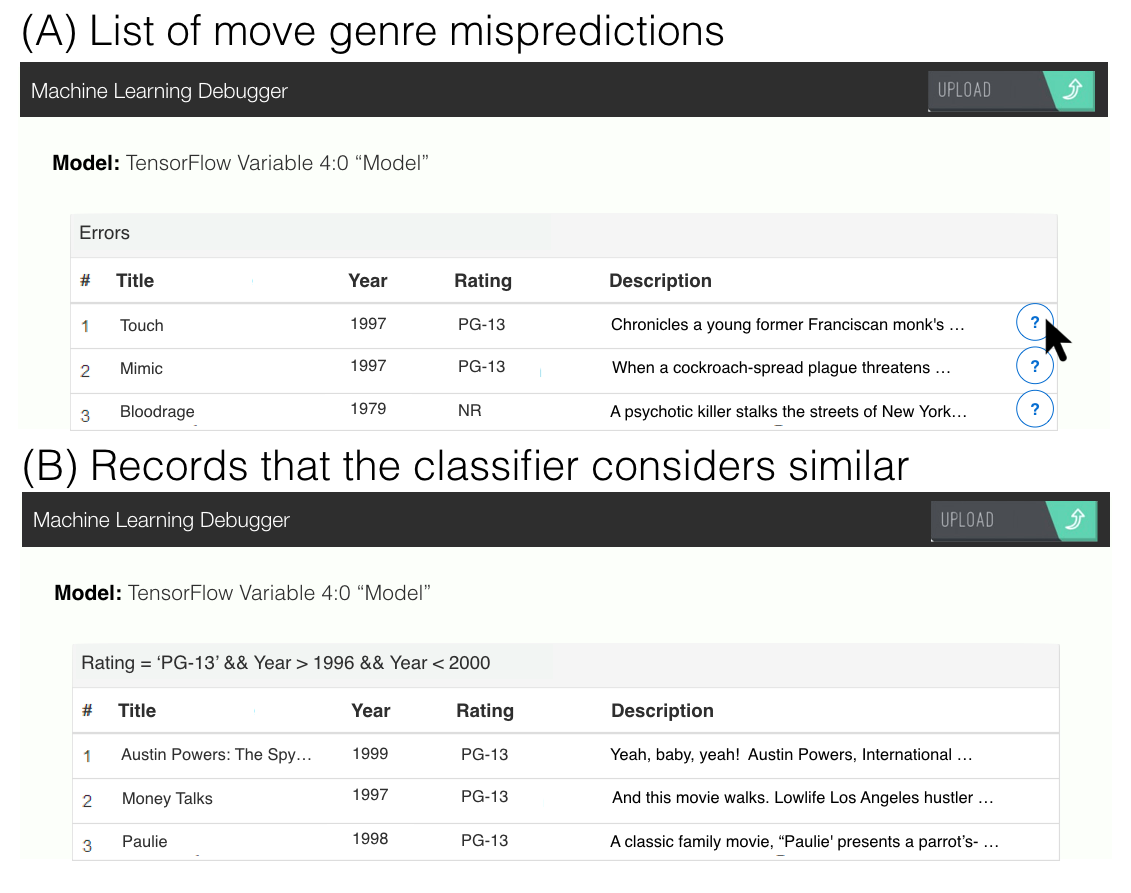
\includegraphics[width=0.6\textwidth]{figures/interface.png}
    \caption{A prototype interface implementing the algorithm. In (A), the interface lists a set tuples that were mis-predicted. Users can dig deeper by selecting one such tuple. (B) is the following panel which describes a predicate and records that the classifier considers as similar.}
    \label{fig:interface}
\end{figure*}